% !TEX root = ./document.tex

\documentclass{article}

\usepackage{mystyle}
\usepackage{myvars}

%-----------------------------

\begin{document}

  \maketitle

  %-----------------------------
  %  TEXT
  %-----------------------------

  \part{Ejercicio Kutner:\\ Mantenimiento de Copiadoras}



    \setcounter{section}{1}
    \setcounter{subsection}{19}
    \subsection{\textbf{Copier maintenance}. The Tri-City Office Equipment Corporation sells an imported copier on a franchise basis and performs preventive maintenance and repair service on this copier. The data below have been collected from 45 recent calls on users to perform routine preventive maintenance service; for each call, $X$ is the number of copiers serviced and $Y$ is the total number of minutes spent by the service person. Assume that first-order regression model \eqref{eq:simple-linear-regression-model} is appropriate.}
    \label{sec:e1-20}

      \begin{equation}
      \label{eq:simple-linear-regression-model}
        Y_i = \beta_0 + \beta_1X_i + \epsilon_i
      \end{equation}

      \subsubsection{Obtain the estimated regression function.}

        \paragraph{}
        [TODO ]

        \begin{figure}[!h]
          \centering
          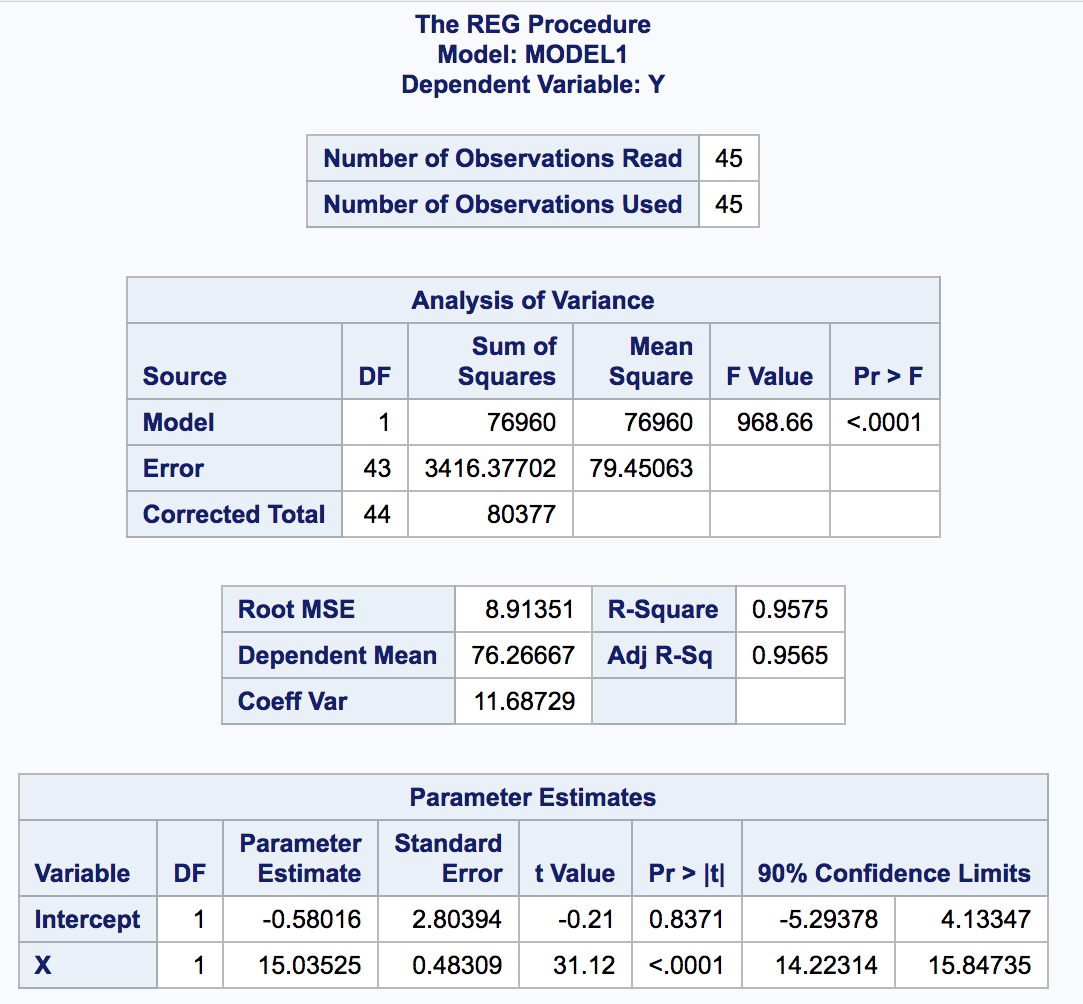
\includegraphics[width=.5\textwidth]{copiers/regression-summary}
          \caption{\emph{Salida SAS}: Mantenimiento de Copiadoras - Resumen de Regresión Lineal Simple}
          \label{img:copiers-regression-summary}
        \end{figure}

        \begin{align}
          \widehat{\beta}_0 &= 0.25419\\
          \widehat{\beta}_1 &= 0.06368\\
          \widehat{Y_i} &= \widehat{\beta}_0 +\widehat{\beta}_1X_i + \epsilon_i = 0.25419 + 0.06368 X_i + \epsilon_i
        \end{align}

      \subsubsection{Plot the estimated regression function and the data. How well does the estimated regression function fit the data?}

        \paragraph{}
        [TODO ]

        \begin{figure}[!h]
          \centering
          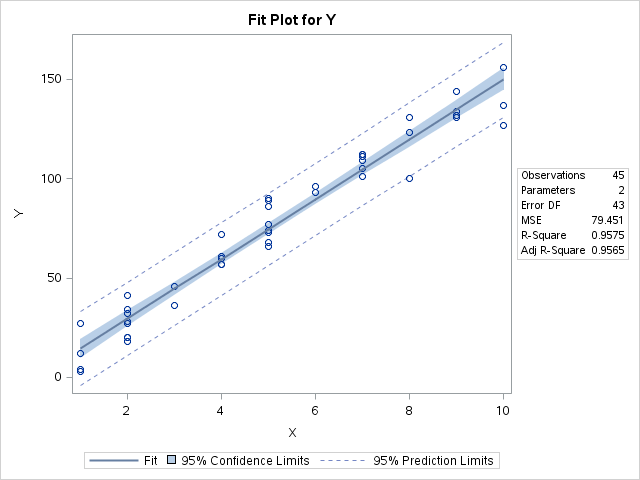
\includegraphics[width=.8\textwidth]{copiers/regression-plot}
          \caption{\emph{Salida SAS}: Mantenimiento de Copiadoras - Gráfico de Regresión Lineal Simple}
          \label{img:copiers-regression-plot}
        \end{figure}

      \subsubsection{Interpret $\widehat{\beta}_0$ in your estimated regression function. Does $\widehat{\beta}_0$ provide any relevant information here? Explain.}

        \paragraph{}
        [TODO ]


      \subsubsection{Obtain a point estimate of the mean service time when $X = 5$ copiers are serviced.}

        \paragraph{}
        [TODO ]

        \begin{figure}[!h]
          \centering
          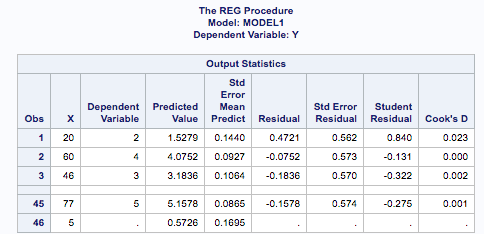
\includegraphics[width=.6\textwidth]{copiers/regression-prediction}
          \caption{\emph{Salida SAS}: Mantenimiento de Copiadoras - Prediccion de Regresión Lineal Simple para $X = 5$}
          \label{img:copiers-regression-prediction}
        \end{figure}

        \begin{align}
          \begin{split}
            E\left[\widehat{Y} \mid X = 5\right] &=
            E\left[\widehat{\beta}_0 +\widehat{\beta}_1X + \epsilon \mid X = 5\right]
            = 0.25419 + 0.06368 * 5 + 0 = 0.5726
          \end{split}\\
          \begin{split}
            Var\left[\widehat{Y} \mid X = 5\right] &=
            \sigma^2\left(1 + \frac{1}{n} + \frac{(x^* - \bar{x})^2}{S_{xx}}\right) =
            0.1695 ^ 2 =
            0.02873025
          \end{split}
        \end{align}

    \setcounter{subsection}{23}
    \subsection{Refer to \textbf{Copier maintenance} Problem \ref{sec:e1-20}.}

      \paragraph{}
      [TODO ]

      \subsubsection{Obtain the residuals $e_i$ and the sum of the squared residuals $\sum_i e_i^2$. What is the relation between the sum of the squared residuals here and the quantity $Q$ in \eqref{eq:least-squares-criterion}?}

        \begin{figure}[!h]
          \centering
          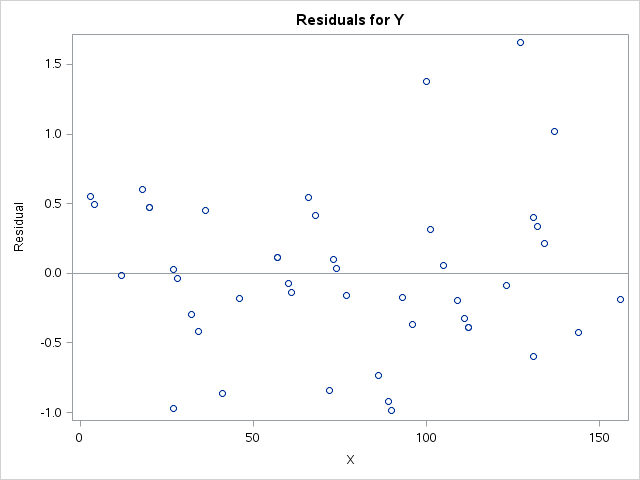
\includegraphics[width=.8\textwidth]{copiers/regression-residuals}
          \caption{\emph{Salida SAS}: Mantenimiento de Copiadoras - Gráfico de Residuos de Regresión Lineal Simple}
          \label{img:copiers-regression-residuals}
        \end{figure}

        \begin{align}
        \label{eq:least-squares-criterion}
          Q &= \sum\limits_{i=1}^n(Y_i - \beta_0 - \beta_1X_i)^2 = 14.47043
        \end{align}


        \paragraph{}
        [TODO ]

      \subsubsection{Obtain point estimates of $\sigma^2$ and $\sigma$. In what units is $\sigma$ expressed?}

        \paragraph{}
        [TODO $\sigma$ en las unidades de $Y$]

        \begin{align}
          \begin{split}
            \widehat{\sigma}^2 &= MSE = \frac{SSE}{n-2} = \frac{\sum_{i=1}^n(Y_i - \widehat{Y}_i)^2}{n-2} = \frac{14.47043}{45-2} = 0.33652
          \end{split} \\
          \begin{split}
            \widehat{\sigma} &= \sqrt{\widehat{\sigma}^2} = \sqrt{0.33652} = 0.58010
          \end{split}
        \end{align}

    \setcounter{section}{2}
    \setcounter{subsection}{4}
    \subsection{Refer to \textbf{Copier maintenance} Problem \ref{sec:e1-20}.}

      \paragraph{}
      [TODO ]

      \subsubsection{Estimate the change in the mean service time when the number of copiers serviced increases by one. Use a $90\%$ confidence interval. Interpret your confidence interval.}
      \label{sec:copiers-2.5a}
        \paragraph{}
        [TODO ]

      \subsubsection{Conduct a \emph{t-test} to determine whether or not there is a linear association between $X$ and $Y$ here; control the $\alpha$ risk at $0.10$. State the alternatives, decision rule, and conclusion. What is the \emph{P-value} of your test?}
      \label{sec:copiers-2.5b}

        \paragraph{}
        [TODO ]

      \subsubsection{Are your results in parts (\ref{sec:copiers-2.5a}) and (\ref{sec:copiers-2.5b}) consistent? Explain.}

        \paragraph{}
        [TODO ]

      \subsubsection{The manufacturer has suggested that the mean required time should not increase by more
than $14$ minutes for each additional copier that is serviced on a service call. Conduct a test to decide whether this standard is being satisfied by Tri-City. Control the risk of a Type I error at $0.05$. State the alternatives, decision rule, and conclusion. What is the \emph{P-value} of the test?}

        \paragraph{}
        [TODO ]

      \subsubsection{Does $\widehat{\beta}_0$ give any relevant information here about the start-up time on calls-i.e., about the time required before service work is begun on the copiers at a customer location?}

        \paragraph{}
        [TODO ]

    \setcounter{subsection}{13}
    \subsection{Refer to \textbf{Copier maintenance} Problem \ref{sec:e1-20}.}

      \paragraph{}
      [TODO ]

      \subsubsection{Obtain a $90\%$ confidence interval for the mean gervice time on calls in which six copiers are serviced. Interpret your confidence interval.}
      \label{sec:copiers-2.14a}

        \paragraph{}
        [TODO ]

      \subsubsection{Obtain a $90\%$ prediction interval for the service time on the next call in which six copiers are serviced. Is your prediction interval wider than the corresponding confidence interval in part (\ref{sec:copiers-2.14a})? Should it be?}

        \paragraph{}
        [TODO ]

    \setcounter{subsection}{23}
    \subsection{Refer to \textbf{Copier maintenance} Problem \ref{sec:e1-20}.}


      \paragraph{}
      [TODO ]

      \setcounter{subsubsection}{1}
      \subsubsection{Conduct an \emph{F-test} to determine whether or not there is a linear association between time spent and number of copiers serviced; use $\alpha = 0.1$. State the alternatives, decision rule, and conclusion.}

        \paragraph{}
        [TODO ]

      \subsubsection{By how much, relatively, is the total variation in number of minutes spent on a call-reduced when the number of copiers serviced is introduced into the analysis? Is this a relatively small or large reduction? What is the name of this measure?}

        \paragraph{}
        [TODO ]

      \subsubsection{Calculate $r$ and attach the appropriate sign.}

        \paragraph{}
        [TODO ]


  \part{Ejercicios Montgomery:}

    \paragraph{}
    [TODO ]


  \part{Código Fuente}

    \begin{figure}[!h]
      \centering
      \begin{minted}[frame=single,framesep=5pt]{sas}
filename reffile '/folders/myshortcuts/sas/regression-group-task/data/CH01PR20.csv';

proc import datafile=reffile dbms=csv out=copiers;
  getnames=yes;
run;

proc print data=copiers;
run;
      \end{minted}
      \caption{\emph{Código SAS:} Mantenimiento de Copiadoras - Importación del conjunto de datos.}
      \label{code:sas-copiers-1}
    \end{figure}


    \begin{figure}[!h]
      \centering
      \begin{minted}[frame=single,framesep=5pt]{sas}
proc reg data=copiers;
  model y=x;
  id x;
run;
      \end{minted}
      \caption{\emph{Código SAS:} Mantenimiento de Copiadoras - Modelo de regresión simple.}
      \label{code:sas-copiers-2}
    \end{figure}

    \begin{figure}[!h]
      \centering
      \begin{minted}[frame=single,framesep=5pt]{sas}
data copiers_new_observation;
  x = 5;
run;

proc append base=copiers data=copiers_new_observation;
run;

proc reg data=copiers;
  model y = x /r clm;
  id x;
run;
      \end{minted}
      \caption{\emph{Código SAS:} Mantenimiento de Copiadoras - Predicción para $X = 5$.}
      \label{code:sas-copiers-2}
    \end{figure}
  %-----------------------------
  %  Bibliographic references
  %-----------------------------

  \nocite{rano2017}
  \nocite{sas}
  \nocite{neter1996applied}
  \nocite{montgomery2012introduction}

  \bibliographystyle{acm}
  \bibliography{bib}

\end{document}
